\documentclass[border=4pt]{standalone}
\usepackage[T1]{fontenc}
\usepackage{lmodern}
\usepackage{amsmath}
\usepackage{pgfplots}
\pgfplotsset{compat=1.18}
\usepgfplotslibrary{groupplots,fillbetween}
\usetikzlibrary{calc,arrows.meta}
% one colour per kind of method, the same in every figure (Okabe-Ito)
\definecolor{neur}{HTML}{D55E00}   % neurons chosen by attribution
\definecolor{dirc}{HTML}{009E73}   % directions from the weird-vs-normal contrast
\definecolor{read}{HTML}{0072B2}   % readout methods and interventions chosen from readouts
\definecolor{pers}{HTML}{CC79A7}   % Assistant Axis / persona
\definecolor{ctrl}{HTML}{8C8C8C}   % random controls
\definecolor{meas}{HTML}{E69F00}   % measured outcome
\definecolor{ink}{HTML}{222222}
\pgfplotsset{
  every axis/.append style={clip=false, font=\small, axis line style={black!55}, tick style={black!55}, tick align=outside,
    label style={font=\small}, tick label style={font=\footnotesize}, title style={font=\small, align=center}},
  grid style={black!9, line width=0.4pt},
  every axis legend/.append style={font=\footnotesize, draw=none, fill=none},
  ci/.style={/pgfplots/error bars/x dir=both, /pgfplots/error bars/x explicit, /pgfplots/error bars/error bar style={line width=0.8pt}, /pgfplots/error bars/error mark=none},
  yci/.style={/pgfplots/error bars/y dir=both, /pgfplots/error bars/y explicit, /pgfplots/error bars/error bar style={line width=0.8pt}, /pgfplots/error bars/error mark=none},
}

\begin{document}
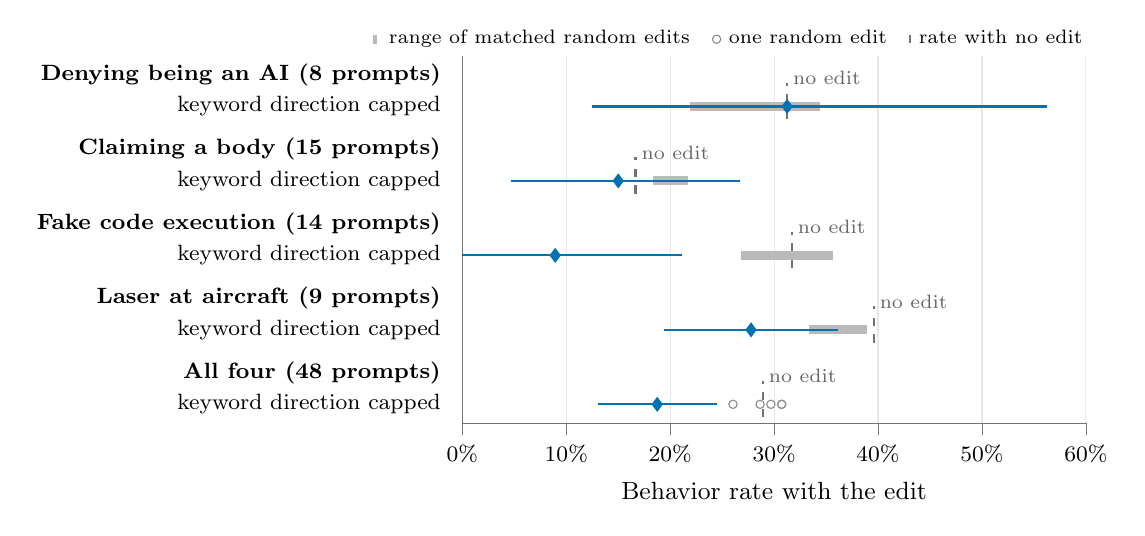
\begin{tikzpicture}
\begin{axis}[width=9.5cm, height=6.25cm, ymin=-11.00, ymax=0.6, ytick={0.00,-1.00,-2.35,-3.35,-4.70,-5.70,-7.05,-8.05,-9.40,-10.40}, yticklabels={{\textbf{Denying being an AI (8 prompts)}},{keyword direction capped},{\textbf{Claiming a body (15 prompts)}},{keyword direction capped},{\textbf{Fake code execution (14 prompts)}},{keyword direction capped},{\textbf{Laser at aircraft (9 prompts)}},{keyword direction capped},{\textbf{All four (48 prompts)}},{keyword direction capped}}, y tick label style={font=\footnotesize}, major y tick style={draw=none}, axis y line*=left, axis x line*=bottom, xmajorgrids, xmin=0, xmax=60, xticklabel={$\pgfmathprintnumber{\tick}\%$}, xlabel={Behavior rate with the edit}]
\draw[black!55, dashed, line width=0.8pt] (axis cs:31.25,-1.40) -- (axis cs:31.25,-0.25);
\node[font=\scriptsize, black!60, anchor=west, inner sep=2pt] at (axis cs:31.25,-0.10) {no edit};
\draw[black!55, dashed, line width=0.8pt] (axis cs:16.67,-3.75) -- (axis cs:16.67,-2.60);
\node[font=\scriptsize, black!60, anchor=west, inner sep=2pt] at (axis cs:16.67,-2.45) {no edit};
\draw[black!55, dashed, line width=0.8pt] (axis cs:31.70,-6.10) -- (axis cs:31.70,-4.95);
\node[font=\scriptsize, black!60, anchor=west, inner sep=2pt] at (axis cs:31.70,-4.80) {no edit};
\draw[black!55, dashed, line width=0.8pt] (axis cs:39.58,-8.45) -- (axis cs:39.58,-7.30);
\node[font=\scriptsize, black!60, anchor=west, inner sep=2pt] at (axis cs:39.58,-7.15) {no edit};
\draw[black!55, dashed, line width=0.8pt] (axis cs:28.91,-10.80) -- (axis cs:28.91,-9.65);
\node[font=\scriptsize, black!60, anchor=west, inner sep=2pt] at (axis cs:28.91,-9.50) {no edit};
\draw[ctrl!60, line width=3.2pt] (axis cs:21.88,-1.00) -- (axis cs:34.38,-1.00);
\addplot[only marks, mark=diamond*, mark size=2.4pt, read, ci] coordinates {(31.25,-1.00) += (25.00,0) -= (18.75,0)};
\draw[ctrl!60, line width=3.2pt] (axis cs:18.33,-3.35) -- (axis cs:21.67,-3.35);
\addplot[only marks, mark=diamond*, mark size=2.4pt, read, ci] coordinates {(15.00,-3.35) += (11.67,0) -= (10.31,0)};
\draw[ctrl!60, line width=3.2pt] (axis cs:26.79,-5.70) -- (axis cs:35.71,-5.70);
\addplot[only marks, mark=diamond*, mark size=2.4pt, read, ci] coordinates {(8.93,-5.70) += (12.22,0) -= (8.93,0)};
\draw[ctrl!60, line width=3.2pt] (axis cs:33.33,-8.05) -- (axis cs:38.89,-8.05);
\addplot[only marks, mark=diamond*, mark size=2.4pt, read, ci] coordinates {(27.78,-8.05) += (8.33,0) -= (8.34,0)};
\addplot[only marks, mark=o, mark size=1.5pt, ctrl] coordinates {(28.65,-10.40) (30.73,-10.40) (30.73,-10.40) (26.04,-10.40) (29.69,-10.40)};
\addplot[only marks, mark=diamond*, mark size=2.4pt, read, ci] coordinates {(18.75,-10.40) += (5.73,0) -= (5.73,0)};
\node[font=\scriptsize, anchor=south east, align=right, inner sep=1pt] at (axis cs:60,0.75) {\tikz\draw[ctrl!60, line width=3.2pt] (0,0) -- (0.4,0); range of matched random edits\quad \tikz\draw[ctrl] (0,0) circle (1.5pt); one random edit\quad \tikz\draw[black!55, dashed, line width=0.8pt] (0,-0.1) -- (0,0.15); rate with no edit};
\end{axis}
\end{tikzpicture}
\end{document}
